% !TeX root = Report.tex
\section{Results}

\subsection{Methodology}

In our simulations we tested networks of various sizes (15, 30 and 48 nodes) aligned in a grid. The nodes were placed such that every node had four neighbours, one to the north, south, east and west, except for nodes in the edge which had three neighbours and the nodes in the corner that had two neighbours. The sink was always placed in the top left corner and was always assigned the address ``1.0''. The predicate checking algorithm was started as soon as the nodes had come online, the nodes then waited for 5 minutes to allow the predicate checking algorithm time to setup and then the TDMA algorithm was started. The simulation was run for 35 minutes overall and then it was terminated. After the predicate checking algorithm had setup the predicate was checked every 4 minutes.

To gather metrics on the energy usage of the motes, a Contiki library called rimestats was used. This library is built into the MAC layer and records deep statistics, we simply used the sent and received message counts. In order to calculate how much energy the TDMA algorithm was using we implemented our own sent and received counters that were incremented when a message was sent or received. As the TDMA protocol was implemented with simple broadcasts there should be a one-to-one correspondence between the number of successful broadcasts and the number of transmissions done at the MAC layer, the same is also true for when receiving a message. To calculate the energy cost of the predicate evaluation algorithm, the difference between the total and the TDMA energy usage was taken.

To check that a predicate was successfully evaluated the TDMA algorithm printed any changes in the assigned slot as well as the time the slot was changed. When a predicate was evaluated on a node the time it was evaluated as well as the result was printed. Analysis scripts then evaluated the predicate using the most recent slot value from before or up to when the predicate was evaluated to evaluate the predicate itself. This result was then compared with the actual result of the predicate. The results were compared whether or not the predicate response message reached the sink.


\subsection{Graphs}

\begin{figure}[ht]
\centering
\subfigure[Rx]{%
	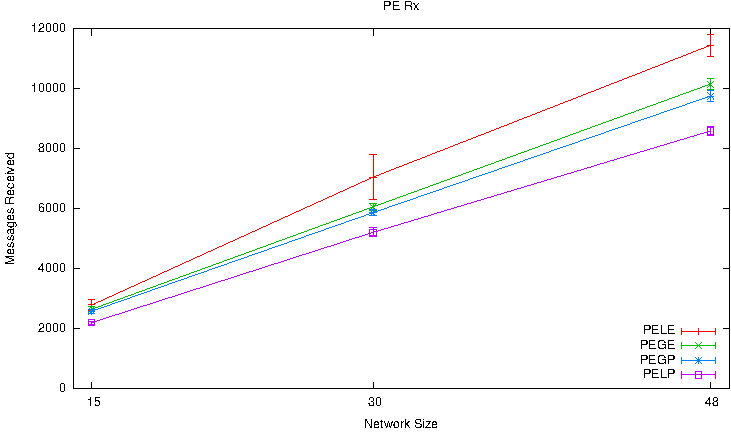
\includegraphics[width=0.44\linewidth]{../Results/Graphs/4.0/1HOP/messagesPE/rx/graph.pdf}
	\label{fig:predeval4.0-rx}
}
\subfigure[Tx]{%
	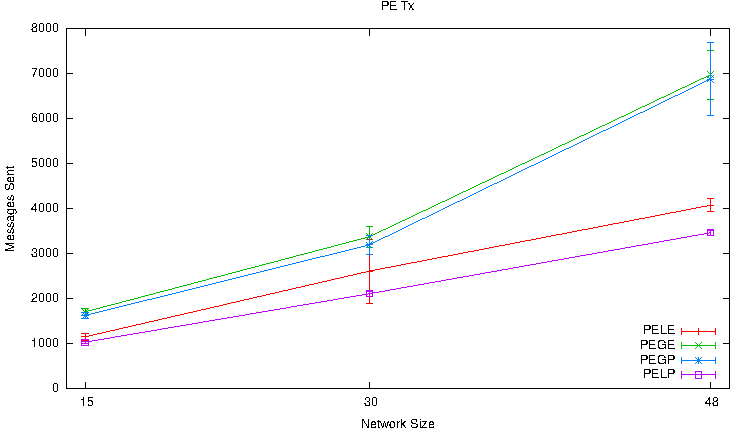
\includegraphics[width=0.44\linewidth]{../Results/Graphs/4.0/1HOP/messagesPE/tx/graph.pdf}
	\label{fig:predeval4.0-tx}
}

\subfigure[Percentage of  predicates correctly evaluated]{%
	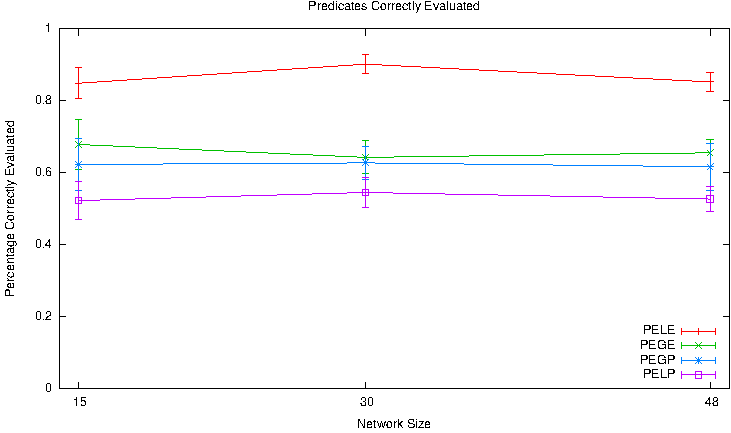
\includegraphics[width=0.44\linewidth]{../Results/Graphs/4.0/1HOP/pcCorrectlyEvaluated/graph.pdf}
	\label{fig:predeval4.0-correct}
}
\subfigure[Percentage of responses received]{%
	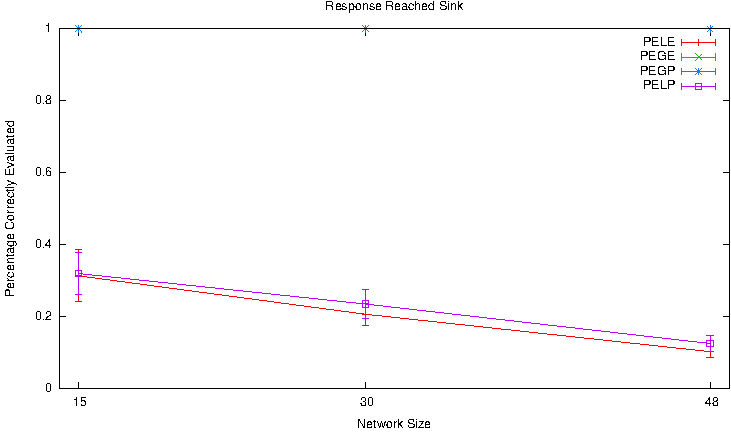
\includegraphics[width=0.44\linewidth]{../Results/Graphs/4.0/1HOP/pcResponsesReachedSink/graph.pdf}
	\label{fig:predeval4.0-recv}
}
\caption{Results when predicate period is every 4.0 seconds using a 1-hop predicate}
\label{fig:predeval4.0}
\end{figure}

The first point of note from the data presented in \autoref{fig:predeval4.0} is that in \subref{fig:predeval4.0-recv}, is that both of the global predicate evaluation algorithms (PEGE and PEGP) show a 100\% delivery rate. While this may initially appear very impressive, this simply arises from the facts that these predicates are evaluated at the sink, and that the graph shows the receipt of evaluated predicates sent from the evaluation location to the sink -- as no messages need to be sent, it is vacuously true that no messages will fail to arrive. The two local predicate checking algorithms, however, showed a more predictable trend of successfully delivering fewer responses as the network size increased, though the specific values of these rates are disappointingly low. The values suggest that only nodes in the immediate environs of the sink are being successful in sending the results of their predicate evaluations (perhaps a consequence of the mesh routing protocol used for sending this information). As the network grows in size, the proportion of nodes within this range of the sink decreases, resulting in the trend shown.

Graph \subref{fig:predeval4.0-correct}, showing the rate of correct predicate evaluation, reveals much more useful information: locally-evaluated event-triggered predicates show significantly higher accuracy than each of the other algorithms. Global event-based predicates was shown to have the second-highest accuracy, though this accuracy was only slightly higher than that of its periodic counterpart so it cannot be concluded that an event-based approach is universally better (within the scope of this metric). There may be a connection between PELE having the highest number of received messages (graph (a)) and its superior accuracy in evaluation; the premise being that more messages being received could give a node more data to use when evaluating a given predicate, in turn making it more likely to return a correct response. This notion of higher message delivery rates for PELE is somewhat corroborated by the number of transmissions shown in \subref{fig:predeval4.0-tx} -- PELE is responsible for the second lowest number messages sent. However, the cause of PELE alone having a significantly higher success rate in delivering messages is as yet unknown, so more definitive information on this front would require further scrutiny using testing methods that may well prove infeasible in a resource-constrained system.

As messages sent and received use the most energy in a WSN system \cite{?} we will use message transmit and receive statistics to evaluate the energy usage of the algorithms. In graphs \subref{fig:predeval4.0-rx} and  \subref{fig:predeval4.0-tx}), local periodic predicate evaluation is the most conservative, however it also shows the lowest accuracy for its evaluations so these results show little in the way of benefits to using this algorithm. By contrast, the most accurate algorithm, PELE, has a higher (yet still moderate) level of energy consumption. An important observation is that the energy demands of global predicate evaluation -- both of which showed middling accuracy -- increase faster than those of local evaluation as network size increases. This is because global evaluation requires data from the entire network, and the operating of the mesh routing protocol means that nodes lying further from the sink will have to have their messages forwarded by a greater number of intermediate nodes, giving exponential growth in the number of messages sent. The local evaluation algorithms show a more scalar trend as the size of a node's 1- or 2-hop neighbourhood may not increase due to the presence of more nodes in the network -- all that is guaranteed is that there will be more such neighbourhoods in which to evaluate predicates.

\begin{figure}[ht]
\centering
\subfigure[Rx]{%
	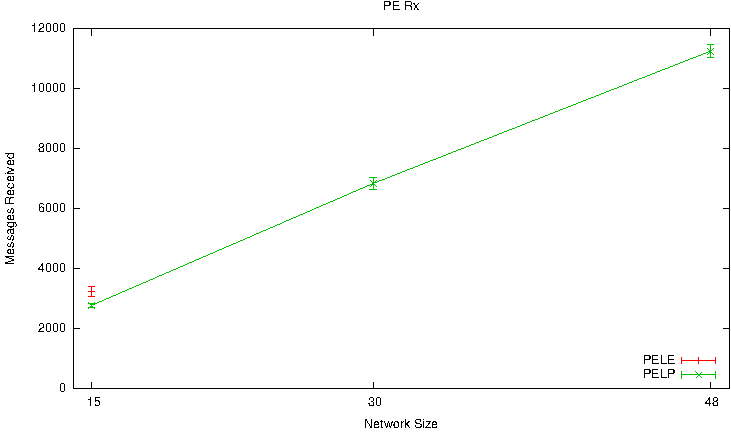
\includegraphics[width=0.44\linewidth]{../Results/Graphs/2.0/1HOP/messagesPE/rx/graph.pdf}
}
\subfigure[Tx]{%
	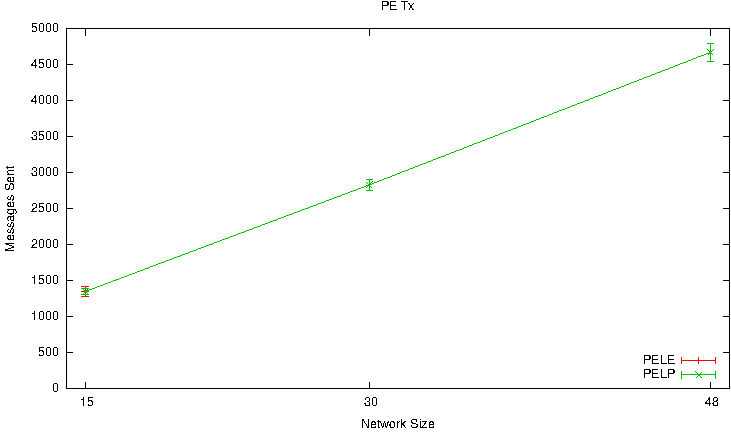
\includegraphics[width=0.44\linewidth]{../Results/Graphs/2.0/1HOP/messagesPE/tx/graph.pdf}
}

\subfigure[Percentage of predicates correctly evaluated]{%
	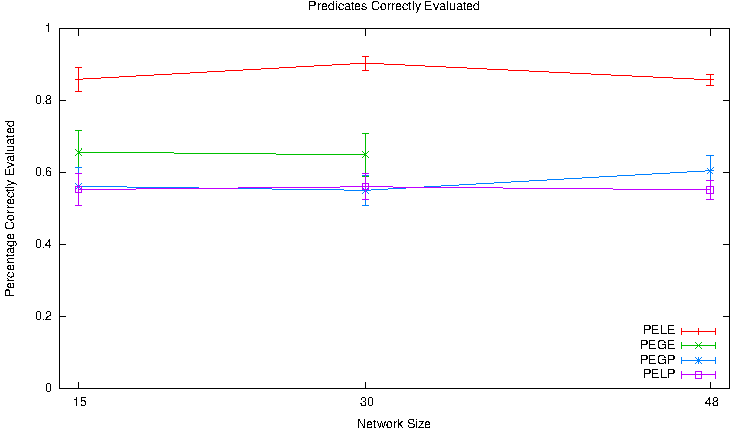
\includegraphics[width=0.44\linewidth]{../Results/Graphs/2.0/1HOP/pcCorrectlyEvaluated/graph.pdf}
}
\subfigure[Percentage of responses received]{%
	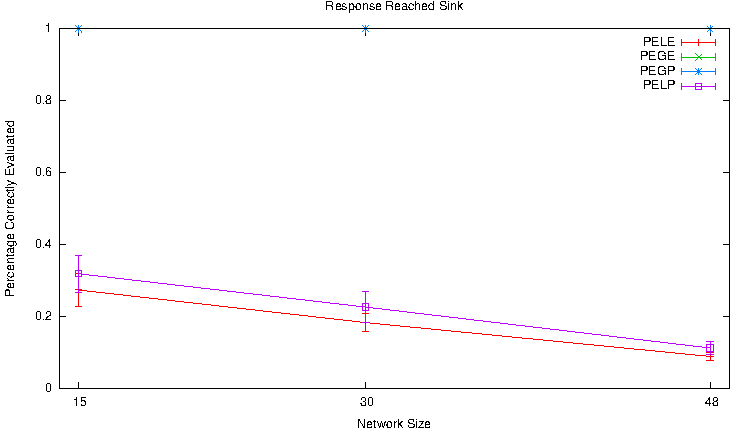
\includegraphics[width=0.44\linewidth]{../Results/Graphs/2.0/1HOP/pcResponsesReachedSink/graph.pdf}
}
\caption{Results when predicate period is every 2.0 seconds using a 1-hop predicate}
\end{figure}

\begin{figure}[ht]
\centering
\subfigure[Rx]{%
	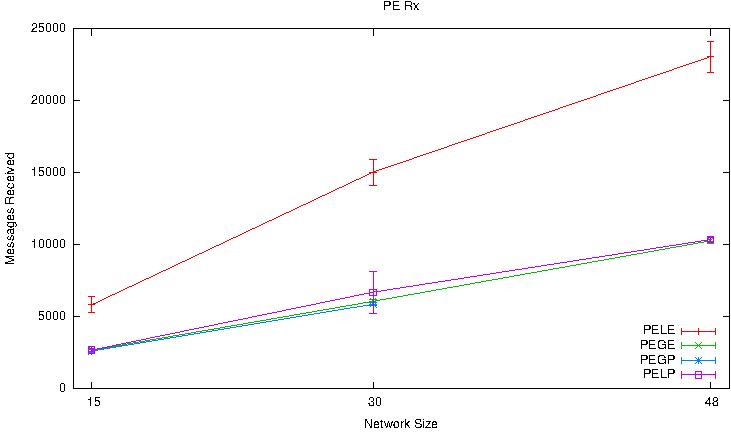
\includegraphics[width=0.44\linewidth]{../Results/Graphs/4.0/2HOP/messagesPE/rx/graph.pdf}
}
\subfigure[Tx]{%
	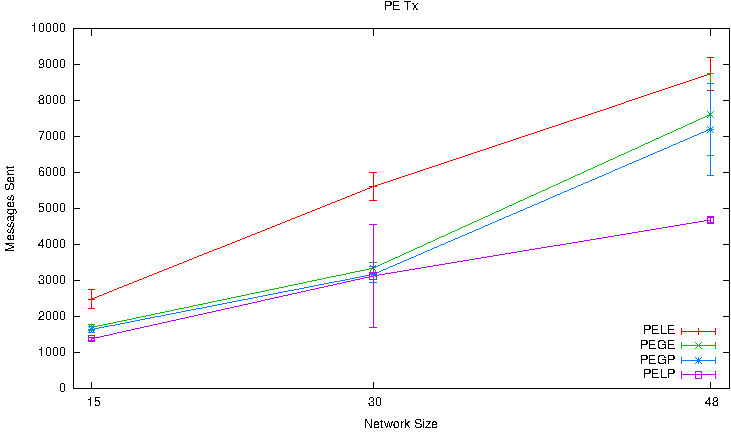
\includegraphics[width=0.44\linewidth]{../Results/Graphs/4.0/2HOP/messagesPE/tx/graph.pdf}
}

\subfigure[Percentage of predicates correctly evaluated]{%
	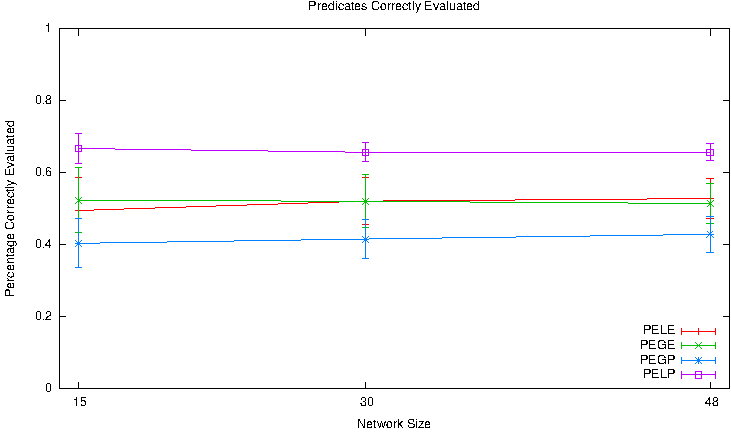
\includegraphics[width=0.44\linewidth]{../Results/Graphs/4.0/2HOP/pcCorrectlyEvaluated/graph.pdf}
}
\subfigure[Percentage of responses received]{%
	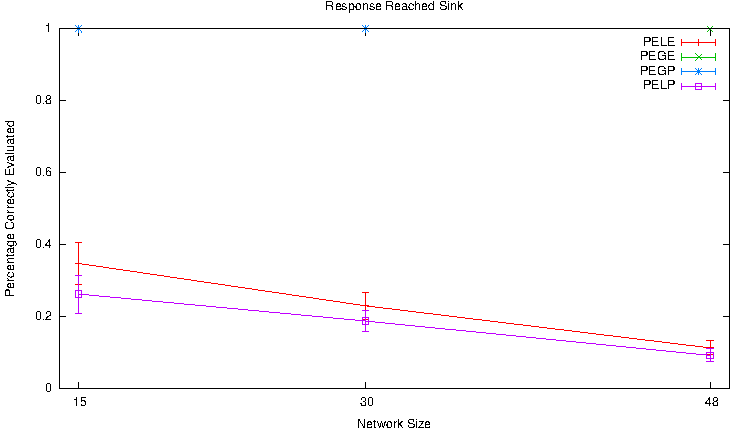
\includegraphics[width=0.44\linewidth]{../Results/Graphs/4.0/2HOP/pcResponsesReachedSink/graph.pdf}
}
\caption{Results when predicate period is every 4.0 seconds using a 2-hop predicate}
\end{figure}

